\documentclass{article}
\usepackage[utf8]{inputenc}
\usepackage{graphicx}

\title{Lab 5 Redes: "Ruteo estático y dinámico"}
\author{Vicente Lopez\\Esteban León\\Sebastian Antón\\Jorge Ramirez\\Profesor: Jose Alejandro Perez\\Ayudante: Alexis Inzunza}
\date{Mayo 2017}

\usepackage{natbib}
\usepackage{graphicx}

\begin{document}
\begin{figure}[h]

\includegraphics[width=0.45\textwidth]{logo_udp.png}
\maketitle
\end{figure}

\section{Indice}
2 Introducción -------------------------------------------------1\\
3 Actividad -----------------------------------------------------1\\
4 Creacion de topologia ------------------------------------ 4\\
5 Conclusión -------------------------------------------------- 5\\
6 Bibliografia -------------------------------------------------- 6\\

\section{Introducción:}
En este laboratorio relizaremos una topologia en cisco packet tracer y la configuraremos con enrutamiento estatico y dinamico identificando sus diferencias.\\\\

\section{Actividad:}
Realice la siguiente topologia en cisco packet tracer:\\\\

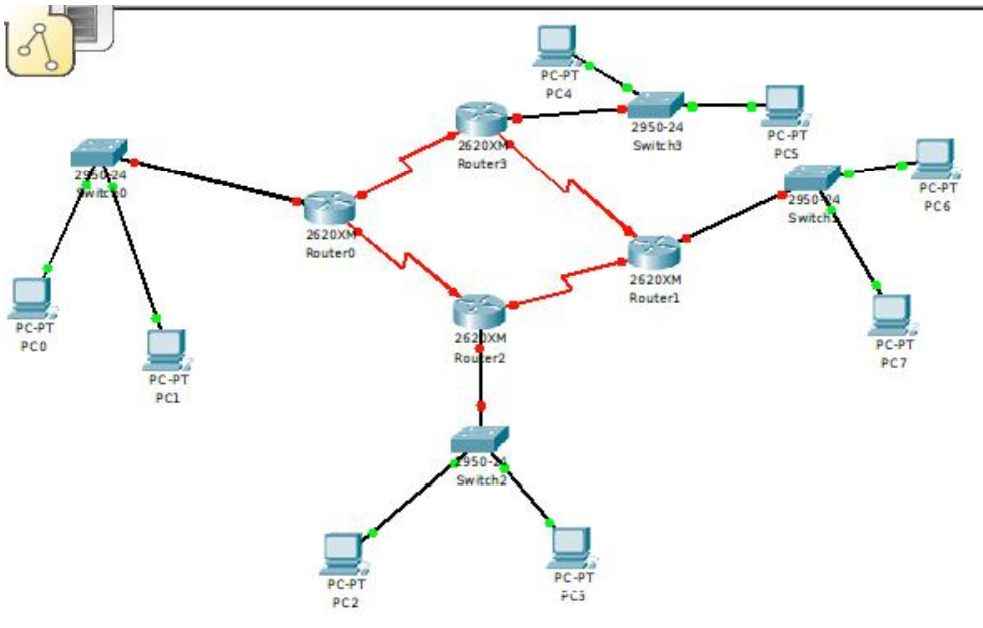
\includegraphics[scale=0.5]{top.png}\\\\

Debido que el router 2620XM cuenta solo con una interfaz, procure apagar el dispositivo
virtual y agregar la interfaz de red WIC-2T y vuelva a encenderlo.\\\\

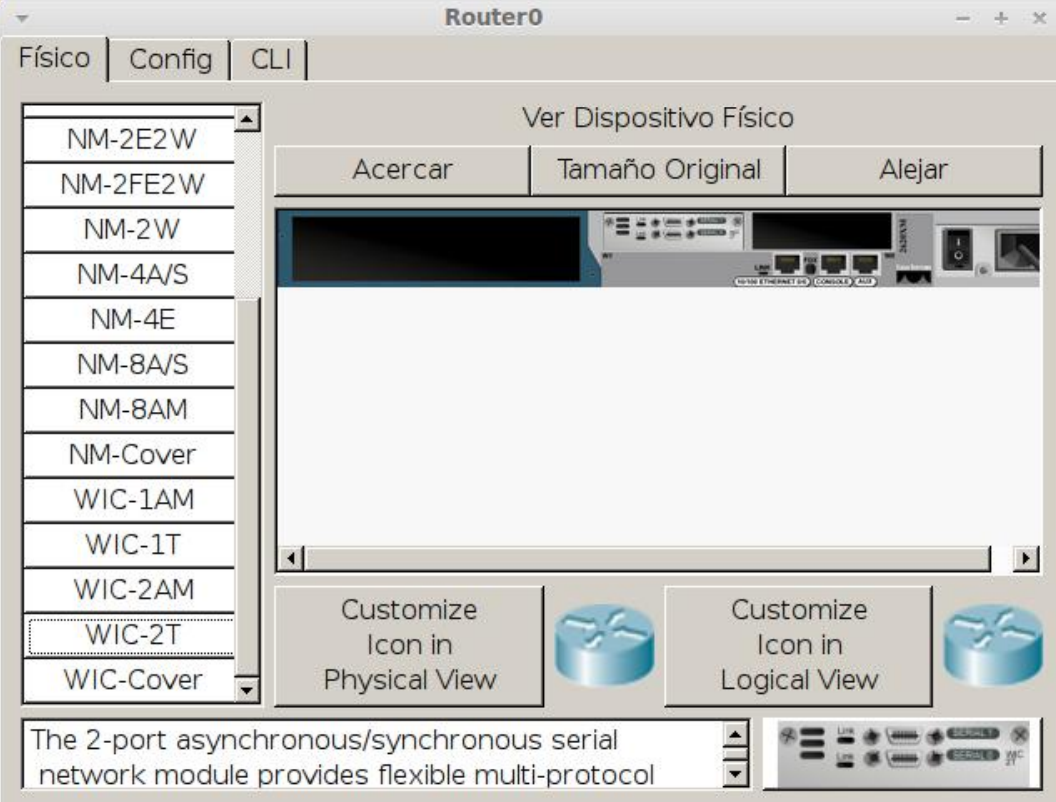
\includegraphics[scale=0.375]{conf.png}\\\\

Asígnele IP manualmente a cada dispositivo y ocupe a su criterio siempre que se cumpla la condición de
que se pueda hacer ping entre todos los equipos. Las configuraciones de ruteo dinámico y estático se realizan
con los comandos que salen a continuación.\\\\\\\\

Configurar tarjeta ethernet del router (la que se conecta con el switch)\\\\

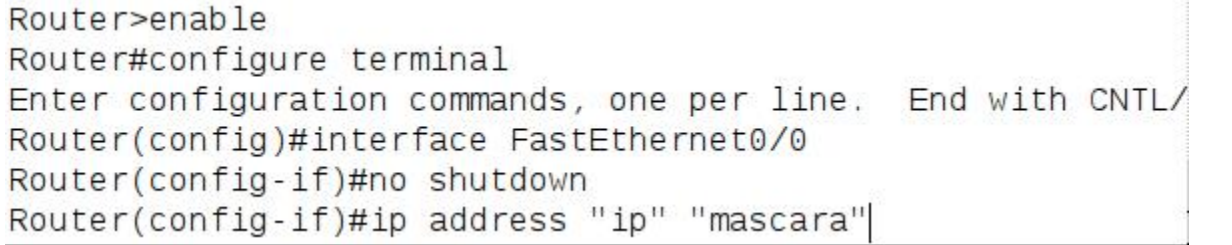
\includegraphics[scale=0.375]{comand1.png}\\\\

Configurar tarjeta serial (recuerde que tiene 2 seriales y una es 0/0 y la otra 0/1)\\\\

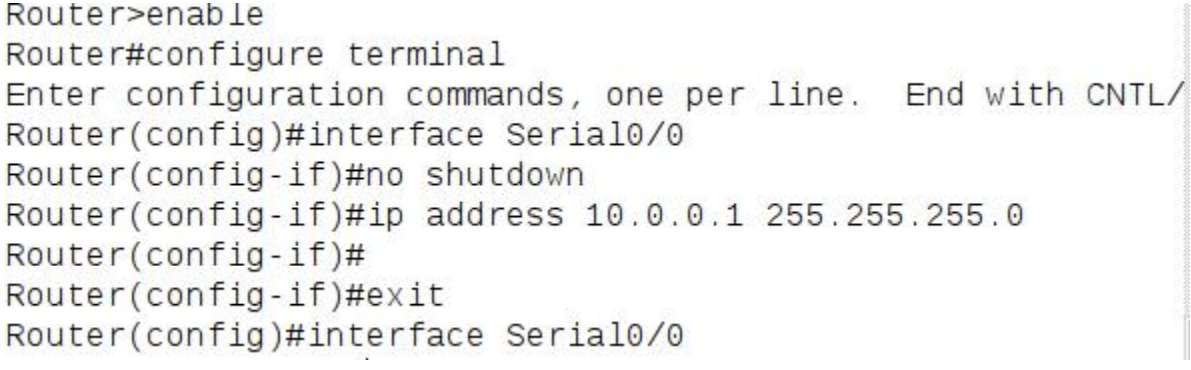
\includegraphics[scale=0.375]{comand2.png}\\\\

Para ruteo Estático\\\\

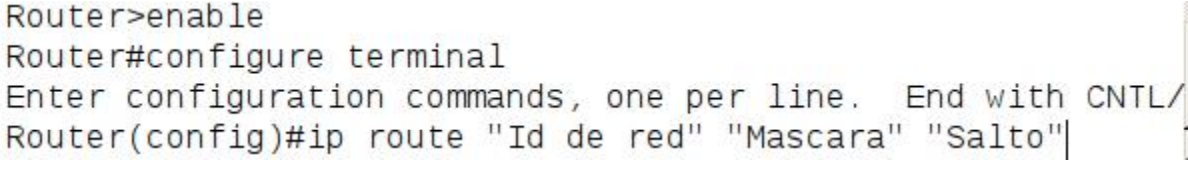
\includegraphics[scale=0.375]{comand3.png}\\\\

Para ruteo Dinámico (usando RIPv2)\\\\

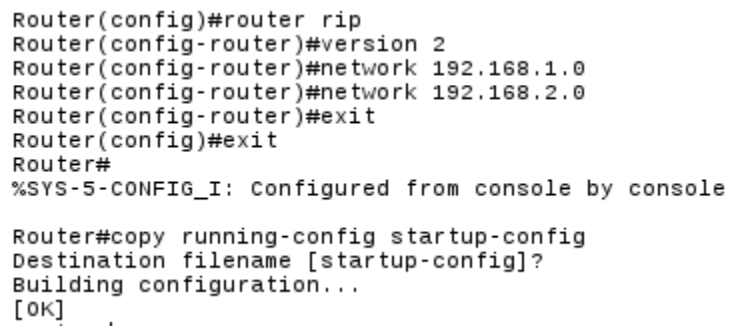
\includegraphics[scale=0.6]{comand4.png}\\\\

En este caso debe cambiar las ip en el comando "network" por aquellas que estén conectadas directamente
al router (no necesariamente son 2).
Realice la topología presentada en la primera página con ruteo dinámico y estático. Debe guardar los
PKT de Cisco Packet Tracer en cada caso y adjuntarlo con su informe.\\\\

\section{Creación de la topologia:}

Como se logra apreciar en la siguiente imagen logramos realizar la topologia solicitada juntos con las configuraciones pedidas:\\\\

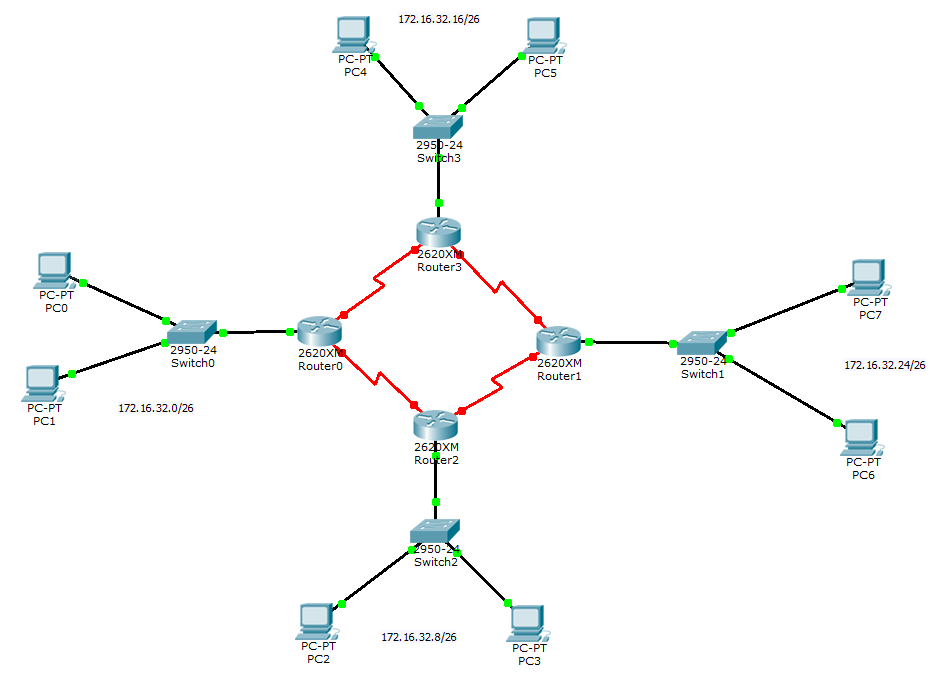
\includegraphics[scale=0.5]{topologia.png}\\\\

y para las direcciones IP de los equipos usamos las siguientes:\\\\

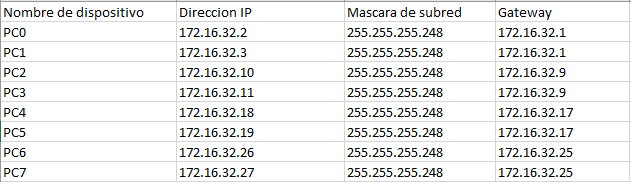
\includegraphics[scale=0.8]{ippc.png}\\\\

\section{Conclusión}
Luego de realizar este laboratorio logramos aprender la realizacion de topologias con enrutamiento estatico y dinamico, y sus respectivas diferencias.\\

Concluimos que el enrutamiento estatico a diferencia del dinamico es mucho más facil de comprender, configurar y mantener redes pequeñas como la de la topologia creada en el experimento, sin embargo, en el enrutamiento dinamico la configuracion es menos propensa a errores y los protocolos reaccionan automaticamente a los cambios de topologia debido a que mantienen actualizada su tabla de enrutamiento a diferencia del estatico, , lo que genera menos intervención por parte de los administradores de la red.\\\\


\section{Bibliografia}
“Redes de Computadoras”, 5a ed, Andrew Tanenbaum y David Wetherall, Pearson Educación, 2012.\\
Laboratorio N5, Ruteo Estático y Dinámico.\\
\end{document}